\documentclass[dvipsnames,t]{beamer}

\usetheme{Madrid}
\usecolortheme[named=RoyalPurple]{structure}

\title{COT3100 Exam 2 review}
\author{Section 1ZED (Carson, Zac)}
\date{Feb 27, 2024}

\begin{document}

\frame{\titlepage}

\AtBeginSection[]
{
\begin{frame}{Topics}
\tableofcontents[currentsection]
\end{frame}
}

\section{Overview}

\begin{frame}{Exam details}
\begin{itemize}
	\item Time: 8:20 to 10:20 PM
	\item Topics:
	\begin{itemize}
		\item 2.3 to 2.5 (no matrices!)
		\item 3.1 to 3.3
		\item Somewhat cumulative (proof techniques, etc.)
	\end{itemize}
	\item Things to bring:
	\begin{itemize}
		\item Writing utensils
		\item Handwritten reference sheet (8.5x11)
		\item 4 function calculator
		\item ID (UF ID, state ID, or ID on phone)
	\end{itemize}
\end{itemize}
\end{frame}

\begin{frame}{Common mistakes!}

\begin{enumerate}
    \item What is the parity of $0$?
    \item List all primes less than $10$.
    \item What is $0!$ ?
    \item What is $\lfloor -3.2 \rfloor$?
\end{enumerate}

\end{frame}

\section{2.3 Functions}

\begin{frame}{Functions}
\begin{block}{Definition}
	A \textit{function} $f$ is written as
	\begin{align*}
	f\colon A \rightarrow B,
	\end{align*}
	where $A$ is the \textit{domain} of $f$ and $B$ is the \textit{codomain} of $f$. Every element of the domain is mapped to exactly one element of the codomain.
\end{block}
\begin{block}{Definition}
	The \textit{range} of a function $f$ is the set of all values of the codomain that are actually mapped to by some value of the domain.
\end{block}
Be careful in using codomain and range! The codomain is the \textit{possible} values that can be mapped to, but they aren't necessarily all mapped to.
\end{frame}

\begin{frame}{One-to-one and onto}
\begin{block}{Definition}
	A function $f$ is \textit{one-to-one} or \textit{injective} if every element of the comain has \textit{at most} one domain element mapped to it.
\end{block}
\begin{block}{Definition}
	A function $f$ is \textit{onto} or \textit{surjective} if every element of the comain has \textit{at least} one domain element mapped to it.
\end{block}
See the relationship?
\end{frame}

\begin{frame}{Bijections}
\begin{block}{Definition}
	A function $f$ is a \textit{one-to-one correspondence} or \textit{bijective} if it is both one-to-one and onto. Equivalently, each codomain element has \textit{exactly one} domain element mapped to it.
\end{block}
\begin{figure}[htp]
    \centering
    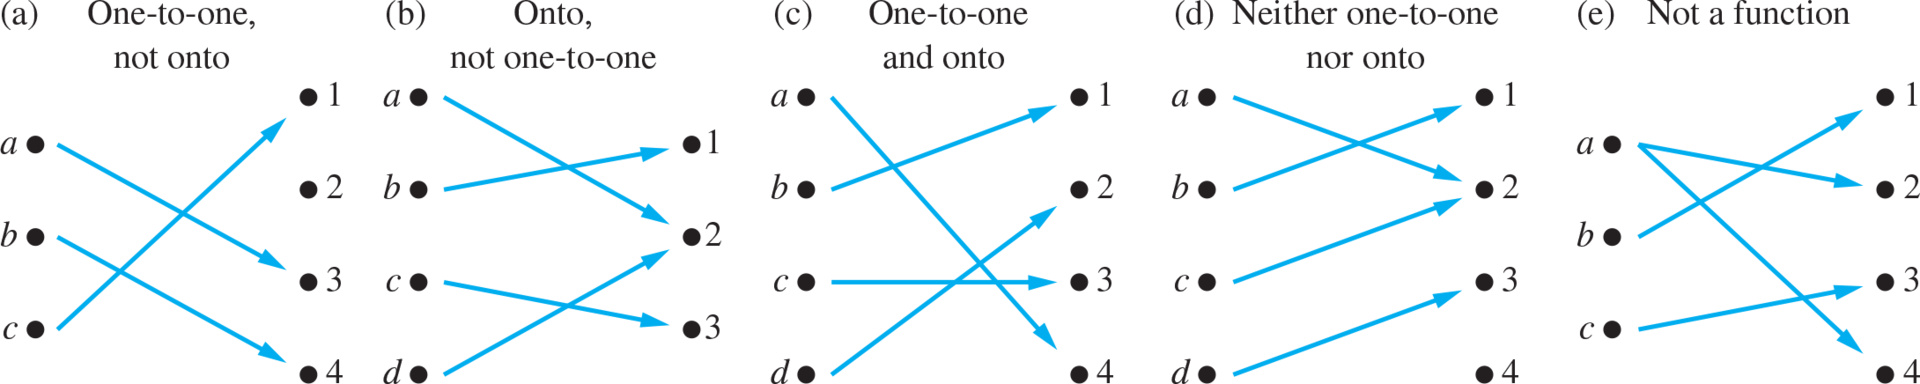
\includegraphics[width=10cm]{func}
\end{figure}
\end{frame}

\begin{frame}{Mathmatical definitions}
\begin{block}{Definition}
	A function $f$ is \textit{one-to-one} if for any two elements $x_1$ and $x_1$ in the domain of $f$,
	\begin{align*}
	f(x_1)=f(x_2) \implies x_1=x_2.
	\end{align*}
\end{block}
\begin{block}{Definition}
	A function $f$ is \textit{onto} if for any element $y$ in the codomain of $f$, there exists an $x$ in the domain where
	\begin{align*}
	f(x)=y.
	\end{align*}
\end{block}

\begin{block}{Note}
	An onto function has the same range and codomain (why?).
\end{block}

\end{frame}

\begin{frame}{Practice}
\begin{block}{Problem}
	Given $f\colon \mathbb{R} \rightarrow \mathbb{R}^+$, where $f(x)=x^4$, prove or disprove if $f$ is one-to-one. Prove or disprove if $f$ is onto. What if the domain was $\mathbb{R}^+$?
\end{block}
\end{frame}

\section{2.4 Sequences and series}

\begin{frame}{Important series}
\begin{align*}
\sum_{i=1}^{n}{i} &= \frac{n(n+1)}{2} \\
\sum_{i=1}^{n}{i^2} &= \frac{n(n+1)(2n+1)}{6} \\
\sum_{i=1}^{n}{i^3} &= \frac{n^2(n+1)^2}{4} \\
\only<1>{\sum_{i=1}^{n}{1} &= \text{?}}
\only<2>{\sum_{i=1}^{n}{1} &= \alert{n}}
\end{align*}
\end{frame}

\begin{frame}{Practice}
\begin{block}{Problem}
	Evaluate
	\begin{align*}
		\sum_{j=0}^{4}{\sum_{k=98}^{100}{\frac{1}{25}(k-97)(j+1)^3}}.
	\end{align*}
\end{block}
\end{frame}

\section{2.5 Cardinality of sets}

\begin{frame}{Countability}
\begin{block}{Definition}
	A \textit{countable} set $S$ has a bijection
	\begin{align*}
	f\colon \mathbb{Z}^+ \rightarrow S.
	\end{align*}
	
	A set where this bijection does not exist is \textit{uncountable}.
\end{block}
\begin{block}{Note}
	The integers $\mathbb{Z}$, the set of even integers, and (surprisingly) the set of rationals $\mathbb{Q}$ are all examples of countable sets.
\end{block}
\begin{block}{Note}
	The set of reals, $\mathbb{R}$ is uncountable. Any interval of $\mathbb{R}$ is also uncountable. The set of irrationals is also uncountable (why?).
\end{block}
\end{frame}


\begin{frame}{Practice}
\begin{block}{Problem}
	Prove that the subset of a countable set is countable.
\end{block}
\end{frame}

\section{3.1 Algorithms}

\begin{frame}{Searching and sorting complexities}
Search algorithms:
\begin{itemize}
\item Linear search - $O(n)$
\item Binary search - $O(\log_2{n})$
\end{itemize}
Sorting algorithms:
\begin{itemize}
\item Bubble sort - $O(n^2)$
\item Selection sort - $O(n^2)$
\item Insertion sort - $O(n^2)$
\end{itemize}

Refer to the textbook and discussion slides for details of each algorithm.
\end{frame}

\begin{frame}{Pseudocode}
When writing pseudocode, getting the message across is most important
\begin{itemize}
\item Will likely look similar to Python
\item Can replace technical syntax (\texttt{array[i][j]=n}) with description (``set array element at $(i,j)$ to $n$'')

\begin{alertblock}{Warning!}<2>
You will likely need to write algorithms beyond searching/sorting!

Be ready to work with arrays (lists), strings, and numbers.
\end{alertblock}
\end{itemize}

\end{frame}

\begin{frame}{Practice}
\begin{block}{Problem}
	For an integer array \texttt{nums} of size at least $2$, let a \textit{peak} be an index $i$ of \texttt{nums} where the element at $i$ is strictly greater than the elements at indices $i-1$ (if it exists) and $i+1$ (if it exists). Describe an algorithm \texttt{peak\_count} that finds the number of peaks of a given \texttt{nums}.
\end{block}
\begin{example}<2>
If \texttt{nums=[2,1,5,3,1]}, then \texttt{nums} has a peak at $i=0$ ($2$) since $2>1$, and a peak at $i=2$ ($5$) since $5>1$ and $5>3$.
\end{example}
\end{frame}

\section{3.2 Growth of functions}

\begin{frame}{Growth rates}
\begin{block}{Note}
The following order represents the growth rates of functions from slowest to fastest:
\begin{align*}
1 \ll \log{n} \ll n \ll n\log{n} \ll n^2 \ll \text{(polynomials)} \ll 2^n \ll n! \ll n^n
\end{align*}
\end{block}
\end{frame}

\begin{frame}{Big $O$}
\begin{block}{Definition}
	A function $f(x)$ is $O(g(x))$ if there are $C$ and $k$ such that
	\begin{align*}
	|f(x)| \leq C|g(x)|
	\end{align*}
	for all $x>k$.
\end{block}
We think of big $O$ as an \textit{upper bound} for the growth of $f$. In other words, $g$ either grows faster or at the same rate as $f$.
\begin{example}<2>
If $f(x)=x^2+3$, then $f(x)$ is $O(x^2)$. However, $f(x)$ is also $O(x^3)$, $O(2^x)$, $O(x!)$, and many more.
\end{example}

\end{frame}

\begin{frame}{Big $\Omega$}
\begin{block}{Definition}
	A function $f(x)$ is $\Omega(g(x))$ if there are $C$ and $k$ such that
	\begin{align*}
	|f(x)| \geq C|g(x)|
	\end{align*}
	for all $x>k$.
\end{block}
We think of big $\Omega$ as a \textit{lower bound} for the growth of $f$. In other words, $g$ either grows slower or at the same rate as $f$.
\begin{example}<2>
If $f(x)=x^2+3$, then $f(x)$ is $\Omega(x^2)$. However, $f(x)$ is also $\Omega(x)$, $\Omega(1)$, etc.
\end{example}
\end{frame}

\begin{frame}{Big $\Theta$}
\begin{block}{Definition}
	A function $f(x)$ is $\Theta(g(x))$ if it is both $O(g(x))$ and $\Omega(g(x))$
\end{block}
We think of big $\Theta$ as giving a ``class'' of functions growing at a similar rate.
\begin{block}{Note}
The ``optimal'' big $O$ refers to the \textit{slowest} growing big $O$ possible. 

Similarly, the ``optimal'' big $\Omega$ refers to the \textit{fastest} growing big $\Omega$ possible. 

These both end up the same as big $\Theta$.
\end{block}
\begin{example}<2>
If $f(x)=x^2+3$, then $f(x)$ is $\Theta(x^2)$. Its ``optimal'' big $O$ and big $\Omega$ are $O(x^2)$ and $\Omega(x^2)$, respectively.
\end{example}
\end{frame}

\begin{frame}{Practice}
\begin{block}{Problem}
Order the following functions of $n$ by their growth rates from \textit{fastest} to \textit{slowest}.
\begin{center}
\begin{tabular}{ cr cr cr cr cr }
(1) & $2024$ & $\alert<2>{(1.0001)^n}$ & $log(n^n)$ & $4n^2-1$ & $n^{2024}$ \\
(2) & $2024$ & $(1.0001)^n$ & $log(n^n)$ & $4n^2-1$ & $\alert<2>{n^{2024}}$ \\
(3) & $2024$ & $(1.0001)^n$ & $log(n^n)$ & $\alert<2>{4n^2-1}$ & $n^{2024}$ \\
(4) & $2024$ & $(1.0001)^n$ & $\alert<2>{log(n^n)}$ & $4n^2-1$ & $n^{2024}$ \\
(5) & $\alert<2>{2024}$ & $(1.0001)^n$ & $log(n^n)$ & $4n^2-1$ & $n^{2024}$
\end{tabular}
\end{center}
\end{block}

\begin{block}{Problem}
For $f(n)=4n^3+n-7$, prove that $f(n)$ is $\Theta(n^3)$.
\end{block}

\end{frame}

\section{3.3 Complexity of algorithms}

\begin{frame}{Practice}
\begin{block}{Problem}
	Find the time complexity of the \texttt{peak\_count} algorithm.
\end{block}
\end{frame}

\end{document}
